\chapter{Mutable objects}
\label{mutable}

\index{String class}
\index{type!String}

As you learned in the previous chapter, an object is a collection of data that provides a set of methods.
For example, a \java{String} is a collection of characters that provides methods like \java{charAt} and \java{substring}.

In this chapter, we explore two new types of objects: \java{Point} and \java{Rectangle}.
We show how to write methods that take objects as parameters and produce objects as return values.

We will also take a first look at the source code for the Java library.


\section{Point objects}
\label{point}

In math, points are often written in parentheses with a comma separating the coordinates.
For example, $(0,0)$ indicates the origin, and $(x,y)$ indicates the point $x$ units to the right and $y$ units up from the origin.

\index{AWT}
\index{java.awt}
\index{Point}
\index{class!Point}

The \java{java.awt} package provides a class named \java{Point} intended to represent the coordinates of a location in a Cartesian plane.
In order to use the \java{Point} class, you have to import it:

\begin{code}
import java.awt.Point;
\end{code}

\index{new}
\index{operator!new}

Then, to create a new point, you have to use the \java{new} operator:

\begin{code}
Point blank;
blank = new Point(3, 4);
\end{code}

\index{declaration}
\index{statement!declaration}

The first line declares that \java{blank} has type \java{Point}.
The second line creates the new \java{Point} with the given arguments as coordinates.

\index{reference}

The result of the \java{new} operator is a {\em reference} to the new object.
So \java{blank} contains a reference to the new \java{Point} object.
Figure~\ref{fig.reference} shows the result.

\index{memory diagram}
\index{diagram!memory}

\begin{figure}[!ht]
\begin{center}
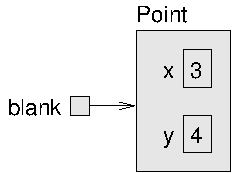
\includegraphics{figs/reference.pdf}
\caption{Memory diagram showing a variable that refers to a \java{Point} object.}
\label{fig.reference}
\end{center}
\end{figure}

As usual, the name of the variable \java{blank} appears outside the box, and its value appears inside the box.
In this case, the value is a reference, which is represented with an arrow.
The arrow points to the \java{Point} object, which contains two variables, \java{x} and \java{y}.

%\section{Attributes}

\index{attribute}
\index{dot notation}

Variables that belong to an object are called {\bf attributes}, but you might also hear them called ``fields''.
To access an attribute of an object, Java uses {\bf dot notation}.
For example:

\begin{code}
int x = blank.x;
\end{code}

The expression \java{blank.x} means ``go to the object \java{blank} refers to, and get the value of the attribute \java{x}.''
In this case, we assign that value to a local variable named \java{x}.

There is no conflict between the local variable named \java{x} and the attribute named \java{x}.
The purpose of dot notation is to identify {\em which} variable you are referring to unambiguously.

You can use dot notation as part of an expression.
For example:

\begin{code}
System.out.println(blank.x + ", " + blank.y);
int sum = blank.x * blank.x + blank.y * blank.y;
\end{code}

The first line displays \java{3, 4}; the second line calculates the value \java{25}.


\section{Objects as parameters}

\index{parameter}
\index{object!as parameter}

You can pass objects as parameters in the usual way.
For example:

\begin{code}
public static void printPoint(Point p) {
    System.out.println("(" + p.x + ", " + p.y + ")");
}
\end{code}

This method takes a point as an argument and displays its attributes in parentheses.
If you invoke \java{printPoint(blank)}, it displays \java{(3, 4)}.

As another example, we can rewrite the \java{distance} method from Section~\ref{distance} so that it takes two \java{Point}s as parameters instead of four \java{double}s.

\begin{code}
public static double distance(Point p1, Point p2) {
    int dx = p2.x - p1.x;
    int dy = p2.y - p1.y;
    return Math.sqrt(dx * dx + dy * dy);
}
\end{code}

Passing objects as parameters makes the source code more readable and less error-prone, because related values are bundled together.

You don't need to write a \java{distance} method, because \java{Point} objects have one built-in already.
To compute the distance between two points, we invoke \java{distance} on one and pass the other as an argument.

\begin{code}
Point p1 = new Point(0, 0);
Point p2 = new Point(3, 4);
double dist = p1.distance(p2);  // dist is 5.0
\end{code}

It turns out you don't need the \java{printPoint} method either.
If you invoke \java{System.out.println(blank)} you get even more information:

\begin{stdout}
java.awt.Point[x=3,y=4]
\end{stdout}

\index{toString}

\java{Point} objects provide a method called \java{toString} that returns a string representation of a point.
When you call \java{println} with objects, it automatically calls \java{toString} and displays the result.
In this case, it shows the name of the type (\java{java.awt.Point}) and the names and values of the attributes.


\section{Objects as return types}

\index{Rectangle}
\index{class!Rectangle}

The \java{java.awt} package also provides a class called \java{Rectangle}.
To use it, you have to import it:

\begin{code}
import java.awt.Rectangle;
\end{code}

\java{Rectangle} objects are similar to points, but they have four attributes: \java{x}, \java{y}, \java{width}, and \java{height}.
The following example creates a \java{Rectangle} object and makes the variable \java{box} refer to it:

\begin{code}
Rectangle box = new Rectangle(0, 0, 100, 200);
\end{code}

Figure~\ref{fig.rectangle} shows the effect of this assignment.

\begin{figure}[!ht]
\begin{center}
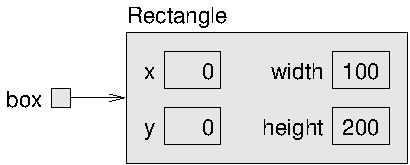
\includegraphics{figs/rectangle.pdf}
\caption{Memory diagram showing a \java{Rectangle} object.}
\label{fig.rectangle}
\end{center}
\end{figure}

If you run \java{System.out.println(box)}, you get:

\begin{stdout}
java.awt.Rectangle[x=0,y=0,width=100,height=200]
\end{stdout}

Again, \java{println} uses the \java{toString} method provided by \java{Rectangle}, which knows how to display \java{Rectangle} objects.

\index{return}
\index{statement!return}

You can write methods that return objects.
For example, \java{findCenter} takes a \java{Rectangle} as an argument and returns a \java{Point} with the coordinates of the center of the rectangle:

\begin{code}
public static Point findCenter(Rectangle box) {
    int x = box.x + box.width / 2;
    int y = box.y + box.height / 2;
    return new Point(x, y);
}
\end{code}

The return type of this method is \java{Point}.
The last line creates a new \java{Point} object and returns a reference to it.

\index{coordinate}

You are probably used to Cartesian {\bf coordinates}, where $x$ and $y$ values can be positive or negative.
In contrast, Java uses a coordinate system where the origin is in the upper-left corner.
That way, $x$ and $y$ are always positive integers.
Figure~\ref{fig.coord} shows these coordinate systems side-by-side.

\begin{figure}[!ht]
\begin{center}
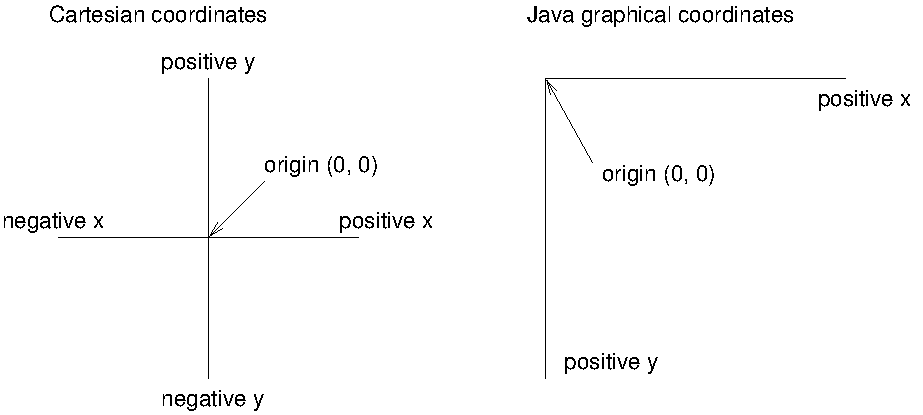
\includegraphics[width=5in]{figs/coordinates.pdf}
\caption{Diagram of the difference between Cartesian coordinates and Java graphical coordinates.}
\label{fig.coord}
\end{center}
\end{figure}

\index{pixel}

Graphical coordinates are measured in {\bf pixels}; each pixel corresponds to a dot on the screen.
You can learn more about Java 2D graphics in Appendix~\ref{graphics}.

The \java{Rectangle} we created using the arguments \java{(0, 0, 100, 200)} has its upper-left corner in the origin.
The center of this rectangle is \java{(50, 100)}, which is 50 pixels to the right and 100 pixels down from the origin.


\section{Rectangles are mutable}

\index{mutable}
\index{object!mutable}

You can change the contents of an object by making an assignment to one of its attributes.
For example, to ``move'' a rectangle without changing its size, you can modify the \java{x} and \java{y} values:

\begin{code}
Rectangle box = new Rectangle(0, 0, 100, 200);
box.x = box.x + 50;
box.y = box.y + 100;
\end{code}

The result is shown in Figure~\ref{fig.rectangle2}.

\begin{figure}[!ht]
\begin{center}
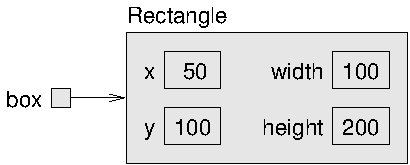
\includegraphics{figs/rectangle2.pdf}
\caption{Memory diagram showing updated attributes.}
\label{fig.rectangle2}
\end{center}
\end{figure}

\index{encapsulation}
\index{generalization}

We can encapsulate this code in a method and generalize it to move the rectangle by any amount:

\begin{code}
public static void moveRect(Rectangle box, int dx, int dy) {
    box.x = box.x + dx;
    box.y = box.y + dy;
}
\end{code}

The variables \java{dx} and \java{dy} indicate how far to move the rectangle in each direction.
Invoking this method has the effect of {\em modifying} the \java{Rectangle} that is passed as an argument.

\begin{code}
Rectangle box = new Rectangle(0, 0, 100, 200);
moveRect(box, 50, 100);
System.out.println(box);  // now at (50, 100, 100, 200)
\end{code}

%The code displays \java{java.awt.Rectangle[x=50,y=100,width=100,height=200]}.

Modifying objects by passing them as arguments to methods can be useful.
But it can also make debugging more difficult, because it is not always clear which method invocations modify their arguments.

Java provides a number of methods that operate on \java{Point}s and \java{Rectangle}s.
For example, \java{translate} has the same effect as \java{moveRect}, but instead of passing the rectangle as an argument, you use dot notation:

\begin{code}
box.translate(50, 100);
\end{code}

This line invokes the \java{translate} method for the object that \java{box} refers to.
As a result, the \java{box} object is updated directly.

\index{object-oriented}

This example is a further illustration of {\bf object-oriented} programming.
Rather than write methods like \java{moveRect} that modify one or more parameters, we apply methods to objects themselves using dot notation.


\section{Aliasing}
\label{aliasing}

\index{reference}

Remember that when you assign an object to a variable, you are assigning a {\em reference} to an object.
It is possible to have multiple variables that refer to the same object.
The memory diagram in Figure~\ref{fig.aliasing} shows the result.

\begin{code}
Rectangle box1 = new Rectangle(0, 0, 100, 200);
Rectangle box2 = box1;
\end{code}

\begin{figure}[!ht]
\begin{center}
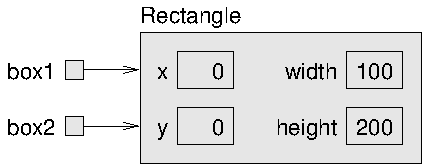
\includegraphics{figs/aliasing.pdf}
\caption{Memory diagram showing two variables that refer to the same \java{Rectangle} object.}
\label{fig.aliasing}
\end{center}
\end{figure}

\index{aliasing}

Notice how \java{box1} and \java{box2} are aliases for the same object, so any changes that affect one variable also affect the other.

This example adds 50 to all four sides of the rectangle, so it moves the corner up and to the left by 50, and it increases the height and width by 100:

\begin{code}
System.out.println(box2.width);   // box2.width is 100
box1.grow(50, 50);                // grow box1 (alias)
System.out.println(box2.width);   // box2.width is 200
\end{code}

The first line displays {\tt 100}, which is the width of the \java{Rectangle} referred to by \java{box2}.
The second line invokes the \java{grow} method on \java{box1}, which stretches the \java{Rectangle} horizontally and vertically.
The effect is shown in Figure~\ref{fig.aliasing2}.

\begin{figure}[!ht]
\begin{center}
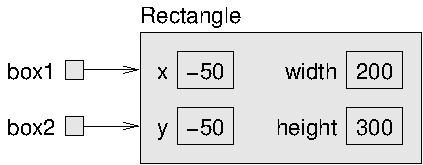
\includegraphics{figs/aliasing2.pdf}
\caption{Memory diagram showing the effect of invoking \java{grow}.}
\label{fig.aliasing2}
\end{center}
\end{figure}

When we make a change using \java{box1}, we see the change using \java{box2}.
Thus, the value displayed by the third line is {\tt 200}, the width of the expanded rectangle.
%(As an aside, it is perfectly legal for the coordinates of a \java{Rectangle} %to be negative.)

%As you can tell from this simple example, code that involves aliasing can get confusing fast, and it can be difficult to debug.
%In general, aliasing should be avoided or used with care.


\section{Java library source}
\label{src.zip}

\index{library}
\index{source code}

Throughout the book, you have used classes from the Java library including \java{System}, \java{String}, \java{Scanner}, \java{Math}, \java{Random}, and others.
You may not have realized that these classes are written in Java.
In fact, you can take a look at the source code to see how they work.

\index{src.zip}

The Java library contains thousands of files, many of which are thousands of lines of code.
That's more than one person could read and understand fully, so don't be intimidated!

Because it's so large, the library source code is stored in a file named \java{src.zip}.
Take a few minutes to locate this file on your computer.
In the paths below, you'll need to replace ``\java{...}'' with the version number.

\begin{itemize}
\item On Linux, it's likely under: \verb"/usr/lib/jvm/openjdk-.../"
\\ If not, then install the {\tt openjdk-...-source} package.
\item On MacOS, it's likely under: \\ \verb"/Library/Java/JavaVirtualMachines/jdk.../Contents/Home/"
\item On Windows, it's likely under: \verb"C:\Program Files\Java\jdk...\"
\end{itemize}

When you open (or unzip) the file, you will see folders that correspond to Java packages.
For example, open the {\tt java} folder, and then open the {\tt awt} folder.
You should now see {\tt Point.java} and {\tt Rectangle.java}, along with the other classes in the \java{java.awt} package.

Open {\tt Point.java} in your editor and skim through the file.
It uses language features we haven't yet discussed, so you probably won't understand every single line.
But you can get a sense of what professional Java source code looks like by browsing through the library.

\index{documentation}
\index{HTML}
\index{Javadoc}

Notice how much of {\tt Point.java} is documentation (see Appendix~\ref{javadoc}).
Each method is thoroughly commented, including \java{@param}, \java{@return}, and other tags.
Javadoc reads these comments and generates documentation in HTML.
You can see the results by reading the documentation for the \java{Point} class, which you can find by doing a web search for ``Java Point''.

Now take a look at the \java{Rectangle} class's \java{grow} and \java{translate} methods.
There is more to them than you may have realized, but that doesn't limit your ability to use these methods in a program.
Object-oriented programming makes it possible to hide messy details so that you can more easily use and understand code that other people wrote.

%By looking at the source code for \java{Point}, \java{Rectangle}, and other classes, we hope you will learn two things.
%1) Objects encapsulate data and provide methods to access and modify the data directly.


\section{Class diagrams}
\label{UML}

To summarize what we've learned so far, \java{Point} and \java{Rectangle} objects each have their own attributes and methods.
Attributes are an object's {\em data}, and methods are an object's {\em code}.
An object's {\em class} defines which attributes and methods it will have.

\index{UML}

In practice, it's more convenient to look at high-level pictures than to examine the source code.
{\bf Unified Modeling Language} (UML) defines a standard way to summarize the design of a class.

\begin{figure}[!ht]
\begin{center}
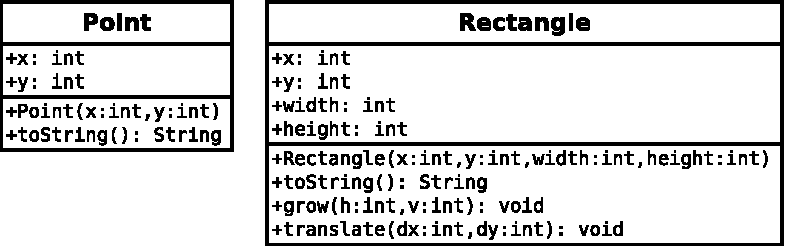
\includegraphics{figs/point-rect.pdf}
\caption{UML class diagrams for \java{Point} and \java{Rectangle}.}
\label{fig.umlPoint}
\end{center}
\end{figure}

\index{class diagram}
\index{diagram!class}

As shown in Figure~\ref{fig.umlPoint}, a {\bf class diagram} is divided into two sections.
The top half lists the attributes, and the bottom half lists the methods.
UML uses a language-independent format, so rather than showing \java{int x}, the diagram uses {\tt x:~int}.

In contrast to memory diagrams, which visualize objects (and variables) at run-time, a class diagram visualizes the source code at compile-time.

Both \java{Point} and \java{Rectangle} have additional methods; we are only showing the ones introduced in this chapter.
See the documentation for these classes to learn more about what they can do.


\section{Garbage collection}

In Section~\ref{aliasing}, we saw what happens when more than one variable refers to the same object.
What happens when {\em no} variables refer to an object?

\begin{code}
Point blank = new Point(3, 4);
blank = null;
\end{code}

The first line creates a new \java{Point} object and makes \java{blank} refer to it.
The second line changes \java{blank} so that instead of referring to the object, it refers to nothing.
In the memory diagram, we remove the arrow between them, as in Figure~\ref{fig.reference3}.

\begin{figure}[!ht]
\begin{center}
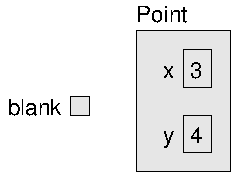
\includegraphics{figs/reference3.pdf}
\caption{Memory diagram showing the effect of setting a variable to \java{null}.}
\label{fig.reference3}
\end{center}
\end{figure}

If there are no references to an object, there is no way to access its attributes or invoke a method on it.
From the program's view, it ceases to exist.
However, it's still present in the computer's memory, taking up space.

\index{garbage collection}

As your program runs, the system automatically looks for stranded objects and deletes them; then the space can be reused for new objects.
This process is called {\bf garbage collection}.
%You can manually run the garbage collector by invoking \java{System.gc()} method.

You don't have to do anything to make garbage collection happen, and in general don't have to be aware of it.
But in high-performance applications, you may notice a slight delay every now and then when Java reclaims space from discarded objects.


\section{Mutable vs immutable}

TODO - StringBuilder example


\section{Vocabulary}

\begin{description}

\term{attribute}
One of the named data items that make up an object.
%Each object has its own copy of the attributes for its class.

\term{dot notation}
Use of the dot operator (\java{.}) to access an object's attributes or methods.

\term{coordinate}
A value that specifies a location in a 2D graphical window.

\term{pixel}
The unit in which coordinates are measured.

\term{object-oriented}
A way of organizing code and data into objects, rather than independent methods.

\term{UML}
Unified Modeling Language, a standard way to draw diagrams for software engineering.

\term{class diagram}
An illustration of the attributes and methods for a class.

\term{garbage collection}
The process of finding objects that have no references and reclaiming their storage space.

\end{description}


\section{Exercises}

The code for this chapter is in the {\tt ch10} directory of {\tt ThinkJavaCode2}.
See page~\pageref{code} for instructions on how to download the repository.
Before you start the exercises, we recommend that you compile and run the examples.

At this point you know enough to read Appendix~\ref{graphics}, which is about simple 2D graphics and animations.
During the next few chapters, you should take a detour to read this appendix and work through the exercises.


\begin{exercise}  %%V6 Ex10.1

The point of this exercise is to make sure you understand the mechanism for passing objects as parameters.

\begin{enumerate}

\item For the following program, draw a stack diagram showing the local variables and parameters of \java{main} and \java{riddle} just before \java{riddle} returns.
Use arrows to show which objects each variable references.

\item What is the output of the program?

\item Is the \java{blank} object mutable or immutable?
How can you tell?

\end{enumerate}

\begin{code}
public static int riddle(int x, Point p) {
    x = x + 7;
    return x + p.x + p.y;
}
\end{code}

\begin{code}
public static void main(String[] args) {
    int x = 5;
    Point blank = new Point(1, 2);

    System.out.println(riddle(x, blank));
    System.out.println(x);
    System.out.println(blank.x);
    System.out.println(blank.y);
}
\end{code}

\end{exercise}


\begin{exercise}  %%V6 Ex10.2

The point of this exercise is to make sure you understand the mechanism for returning new objects from methods.

\begin{enumerate}

\item Draw a stack diagram showing the state of the program just before \java{distance} returns.
Include all variables and parameters, and show the objects those variables refer to.

\item What is the output of this program?
(Can you tell without running it?)

\end{enumerate}

\begin{code}
public static double distance(Point p1, Point p2) {
    int dx = p2.x - p1.x;
    int dy = p2.y - p1.y;
    return Math.sqrt(dx * dx + dy * dy);
}
\end{code}

\begin{code}
public static Point findCenter(Rectangle box) {
    int x = box.x + box.width / 2;
    int y = box.y + box.height / 2;
    return new Point(x, y);
}
\end{code}

\begin{code}
public static void main(String[] args) {
    Point blank = new Point(5, 8);

    Rectangle rect = new Rectangle(0, 2, 4, 4);
    Point center = findCenter(rect);

    double dist = distance(center, blank);
    System.out.println(dist);
}
\end{code}

\end{exercise}


\begin{exercise}  %%V6 Ex10.3

This exercise is about aliasing.
Recall that aliases are two variables that refer to the same object.

\begin{enumerate}

\item Draw a diagram that shows the state of the program just before the end of \java{main}.
Include all local variables and the objects they refer to.

\item What is the output of the program?

\item At the end of \java{main}, are \java{p1} and \java{p2} aliased?
Why or why not?

\end{enumerate}

\begin{code}
public static void printPoint(Point p) {
    System.out.println("(" + p.x + ", " + p.y + ")");
}
\end{code}

\begin{code}
public static Point findCenter(Rectangle box) {
    int x = box.x + box.width / 2;
    int y = box.y + box.height / 2;
    return new Point(x, y);
}
\end{code}

\begin{code}
public static void main(String[] args) {
    Rectangle box1 = new Rectangle(2, 4, 7, 9);
    Point p1 = findCenter(box1);
    printPoint(p1);

    box1.grow(1, 1);
    Point p2 = findCenter(box1);
    printPoint(p2);
}
\end{code}

\end{exercise}
